\documentclass[a4paper]{article}

\usepackage{graphicx}
\usepackage{listings}
\usepackage{color}
\usepackage[margin=0.5in]{geometry}

\begin{document}


\justify

\section{1. Introduction}

Currently, most music production software is a native application, that being, that it does not run on or even require the Internet. The benefits of this is that it allows to be extremely powerful, allowing the software to make full advantage of the computer's capabilities. They often have in-built synthesisers, drum machines and effects units; along with the ability of being able to plug in external machines it allows the client to produce and create any imaginable genre of music. This gave power to the individuals, now anyone with an idea and willingness can learn and create music, regardless of age, money or training. However, even though modern applications strive to make the learning curve as minimal as possible, the use of them to a beginner can be quite daunting. This and the fact that it is near impossible to be able to collaborate on a single music project in real-time unless in the same room give rise to a few, but very important, disadvantages. \par

The rise of the Internet saw a slow and steady increase in web-based applications. Only recently with the advancements and wide acceptance of JavaScript and its in-built capabilities of creating manipulating sound has it really began to move forward. There are a few powerful, in-depth web-based music production tools and a whole host of simple, standalone, web-based synthesisers, drum machines and effect units. However, very few, if not none, make full advantage of the raw capabilities of the internet, communication. I believe there is room for a web-based music production tool that allows for real-time collaboration. The only requirements a user needs is access to the Internet, minimal knowledge of music, how a sequencer works (although should be intuitive enough to pick up without prior knowledge) and someone to create music with. \par

\section{2. Business case}

\subsection{2.1 Background and Motivation}

Music production software has taken many forms since the inception of the computer. They allow clients to write, produce and create all different genres of music, only needing a computer and the software. Modern adaptations strive to make it as easy as possible, with little-to-none prior knowledge of music needed to get going and a wealth of in-built synthesisers and drum machines, often replicating real world tools to a high standard. They can be used in conjunction with external musical hardware such as synthesisers or drum machines by manipulating MIDI signals and are powerful enough to allow the expert user to create best selling albums. However, professional software is very costly and requires a relatively powerful computer to operate effectively on. They also are very solo artist orientated. That meaning, unless in the same room as the producer, it would be near impossible collaborate on the project. \par

Only recently with the wider acceptance of JavaScript with its in-built Web Audio API capabilities that allow for creation and manipulate sound, has web-based music applications have risen. The advantages of having web-based music creation software over bespoke native applications is the same as the advantages of the Internet in general. Anyone with access to the internet can create music as well as allowing collaboration on a world wide scale. The amount of web-based production software, synthesisers, drum machines has steadily been increasing. Most however, are still standalone, that focus on a particular genre or hardware and aren't multi-user focussed. I see that there is a real opportunity to create some music production software that allows for real-time collaboration. This meaning that not only is the access to the software is only restricted by the user having access to the internet, it also allows for two people, from anywhere in the world, to collaborate on the same music project at the same time. It should be intuitive enough for basic users to be able to use it efficiently and have the capabilities for advance users to be able to create and manipulate to a high degree. \par

\subsection{2.2 Business Objectives}

\begin{itemize}
    \item[$\alph$] To allow for collaboration on music projects with two or more people.
    \item[$\alph$] Remove the need to send music projects back and forth or to have to meet up in 'real-life' to collaborate on a music project together.
    \item[$\alph$] To have a basic web-based digital audio workstation for creation of music in with the use of external hardware if wanted.
    \item[$\alph$] To be able to intuitively use the software to create a piece of music without much prior knowledge of how to do so.
    \item[$\alph$] To be able to track, manage and edit created pieces of music.
    \item[$\alph$] Remove the need for an expensive, computationally heavy piece of software to achieve this.


\end{itemize}

\section{3. Project objectives}

\begin{enumerate}
    \item Analyse and current music creation process with music with current musical software to understand the basic needs of musicians working with computers.
    \item User portal to be able to keep information about the user and for them to be able to manage, edit and delete their music projects.
    \item A web-based digital audio workstation that allows for creation of scores of music.
    \item A web-based digital audio workstation has pre-loaded samples that they can use.
    \item Two or more users can simultaneously work on the same project in real-time and see the other's inputs reflected on the project as they happen.
    \item They can manipulate the sound parameters of the samples.
    \item Users can then download their musical composition as an audio file.
    \item An intuitive interface that allows for quick and easy music creation.
\end{enumerate}

\section{4. Initial scope}

I have decided to use the MoSCoW technique in order to measurably define my project requirements. This ranking technique is defined by: M - must have, S - should have, C - could have, W - would have. In order for my project to be defined as successful, it should have met all 'Must have' defined requirements. The numbering in the table below refers to the same number of that requirement defined in the '3. Project objectives' as to expand information on that specific requirement, and any further sub-points will be defined alphabetically.

INSERT PICTURE FROM TABLE

\section{5. Resources and dependencies}

The project isn't currently dependable on any external resources or products. I have provided the server in which it is run which is funded by myself which has all capabilities to host application and database.

I may use the front-end framework 'Express' that is heavily used throughout many NodeJS projects, however this is isn't decided for certain yet and even if so, the project is very stable and with a large following so it wouldn't cause any problems. I am also planning to use the third-party library socket.io to help with the real-time client to server communication. This is because it helps with ease of development and it isn't realistic to create everything myself when suitable alternatives are available. Both frameworks are highly recognised and have a big community surrounding them so they shouldn't cause problems in their failure to be maintained.

REFER(http://expressjs.com/). I will a
REFER(socket.io)


Potentially, for some desirable features, I might use other pre-existing JavaScript library to make development faster. However, I intend to avoid the use of them at all cost throughout my project. If such libraries are used, a document of how they are used and the justification for using will be in the final report as well as weekly summary. \par

\section{6. Method of approach}

After some research I have decided my software development process will follow that of an AGILE approach using SCRUM methods. That is, to release working minimal viable products early and often. This is because I have experience with this process, I know how to plan the work and I would like to get minimal viable products out as soon as possible.

The first stage of iterations will be to get the core product working and usable. I want a step-sequencer that a user can create simply pattern and melody using basic samples.

The second stage of iterations will be to get the operational transformation algorithm in place which allows for the 'real-time collaboration' portion of the program to work.

Once these are in place, that is the core functionality of my web-application done and I would like to focus on incrementally improving the product and adding desirable features.

Possible technologies are NodeJS and within the JavaScript Web Audio API, Express framework and Socket.io library. Also HTML and CSS for all front end styling and layout. I haven't decided whether I will be using a relational database or a NoSQL database yet for storage of samples and potential storage for user's session/work. I need to revise and my data that will be stored and see which suits best. I'm leaning towards a NoSQL approach due to the fact the data will be of different types and if I am storing user sessions the data will be unstructured or at least difficult to restrain into a table. If I do decide to go with a relational database I will use MySQL as I've had previous experience with it, otherwise I will use a document store NoSQL database such as MongoDB. This will be decided upon after the requirement gathering stage of my project as I will have a better idea of what is needed. Git will be used as a versioning mechanism of code base which will be committed to my personal and private GitHub repository. For unit tests I intend to use Mocha.js testing framework as I have had previous experience with it. I will research and try to implement a continuous deployment methodology into my project to ensure streamlined deployment process, complete with unit tests checked before deployment and syncing code to server. I hope to do a mixture of coding styles but enforcing Test driven development when necessary to ensure code clarity and maintainability. For the ability to connect external devices to the application, I will be manipulating MIDI signals from the device using the Web MIDI API as it is the most recognised way to do so.

\section{7. Project plan}

\begin{figure}

    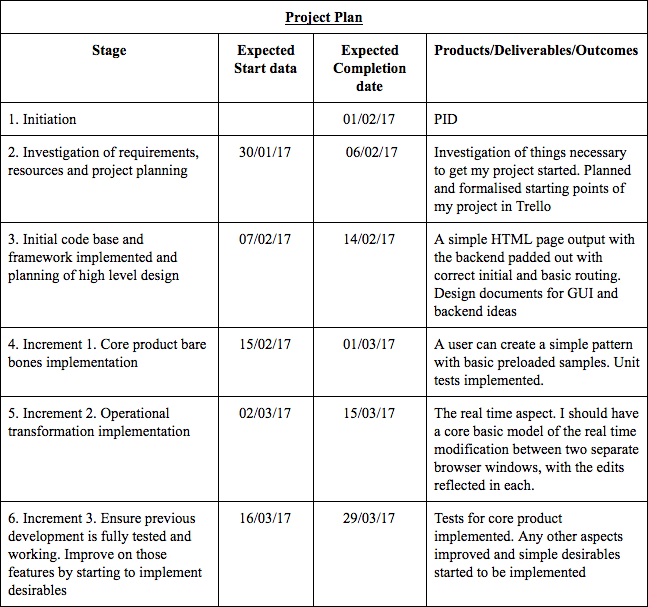
\includegraphics[width=\linewidth]{img/project-plan-table.png}

\end{figure}

\subsection{7.1 Control plan}

\begin{enumerate}
    \item Highlight reports as dictated by the PROC304 module
    \item Review meetings with project supervisor as dictated by the PRCO304 module; additional ad-hoc meetings as and when necessary. Notes of meetings shall be documented.
    \item Risk management (see Section 8); communication plan (see Section 7.2); quality plan (see Section 9); exception reports and plans as necessary
    \item I will use on-line project tracking tool 'Trello' to plan my project. In this I have boards that have general things that are needed for the project and within further columns in which I can move cards, which are more specific tasks to the board, from left to right to track progress. I will also do this to track the work my fortnightly sprints. I will use boards in the following ways:
        \begin{enumerate}
            \item To have board on the project initiation which is what I need to do to get the project at a level where I can start working on the code. This include cards with check-lists for setting up server, bare bones code base, project documents etc.
            \item To have a project backlog board which houses all my project ideas, requirement gathering for them, when requirement gathering is done moves to ready for story point estimation and then finally sprint candidates.
            \item To have a board that tracks my current sprint. This will have columns for Sprint backlog (list of user stories for the sprint), In progress, a column for QA-ing (making sure it hits requirements and further testing of functionality), ready for release and done (a card will move into done when it is deployed). I have an extension to Trello which allows me to assign and track user story points for each user story. This will allow me to refine my assigning which ultimately will give me a better idea for how much work I have and how long it will take. I plan to show progress in a burn down chart.
        \end{enumerate}
 \end{enumerate}

\subsection{7.2 Communication plan}

I have no further stakeholders or real-clients apart from myself and my supervisor. When my product is to a presentable core working prototype, I intend to hold regular meetings to get constant feedback on the product. When I seek feedback from potential users, I will plan meetings with a individuals or groups with a script and make sure the discussion of the meeting is documented fully. Review meetings will be held with the supervisor in line with the Control plan. Further ad-hoc communications will take place as needed. Unexpected outcomes or execptions will be documented and brought to light in the review meeting unless seen as a matter of urgancy.

\section{8. Initial risk list}

\begin{figure}

    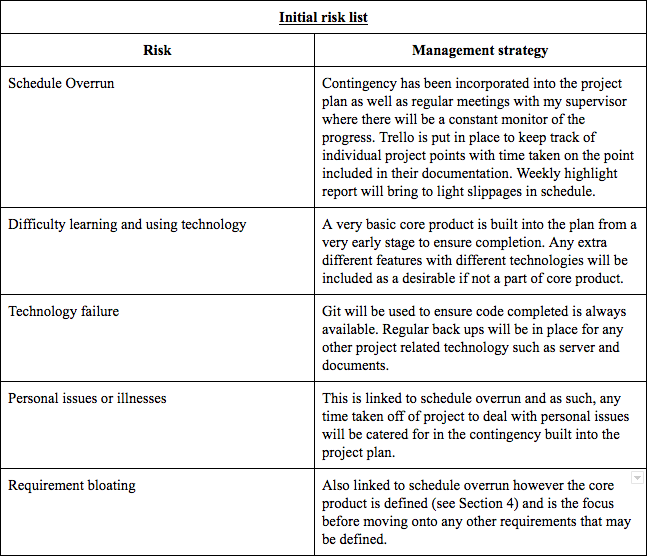
\includegraphics[width=\linewidth]{img/initial-risk-table.png}

\end{figure}

\section{9. Initial quality plan}

\begin{figure}

    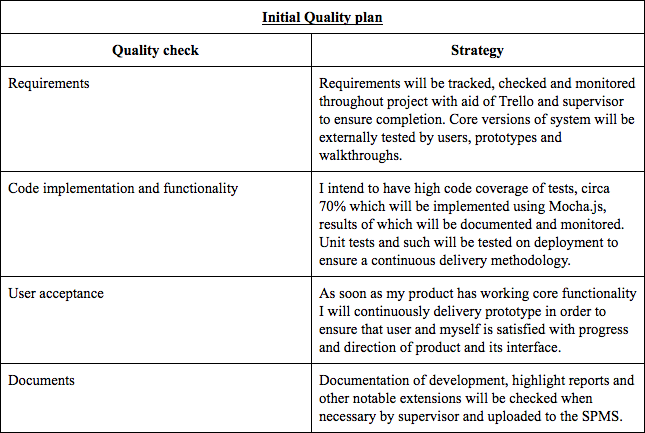
\includegraphics[width=\linewidth]{img/initial-quality-table.png}

\end{figure}

\section{10. Legal, ethical, social and/or professional issues}

Music samples used in the software will be royalty free and free to use completely without copyright infringement to abide by laws. If the functionality to be able to upload own samples is implemented, a disclaimer will be in place to make sure that the user accepts full responsibility for the use of samples that are not royalty free. If the inbuilt text messaging feature is built, I will have to make sure that the user acceptance responsibility for any text communicated in the product. As the user's have to know eachother to share the link one would assume that this won't be a problem, however I believe a monitoring tool inside program is outside of the scope of this project.

\section{Questions}

- Does the project plan table need to have days or just data suffice? \par
- Does my business case need more detail \par
- Do I need more objectives \par
- first section of initial scope to be moved into method approach or control plan? \par
- unit tests as part of objectives? maybe a code coverage metric \par
- Does my project plan outcomes need to be more measurable? \par

\end{document}
